\documentclass{bredelebeamer}
\usepackage{amsfonts}
\usepackage{amsmath}
\usepackage{multirow}
\usepackage{bbm}
\usepackage{xparse}

%% OPTIONS

\graphicspath{{./images/}}
\def\bc{\begin{center}}
\def\ec{\end{center}}
%========================================================
\def\bit{\begin{itemize}}
\def\eit{\end{itemize}}

\def\la{{\langle}}
\def\ra{{\rangle}}
\def\da{\,{\partial_a}}


\def\ind{{\bf 1}}
\def\demi{\frac{1}{2}}

\AtBeginSection[]{
	\begin{frame}
		\vfill
		\centering
		\begin{beamercolorbox}[sep=8pt,center,shadow=true,rounded=true]{title}
			\usebeamerfont{title}\insertsectionhead\par%
		\end{beamercolorbox}
		\vfill
	\end{frame}
}

\newenvironment<>{varblock}[2][.9\textwidth]{%
	\setlength{\textwidth}{#1}
	\begin{actionenv}#3%
		\def\insertblocktitle{#2}%
		\par%
		\usebeamertemplate{block begin}}
	{\par%
		\usebeamertemplate{block end}%
\end{actionenv}}


\def\t{{\texttt{t}}}
\def\logit{\,{\text{logit}}\,}
\def\x{\times}
\def\ox{\otimes}
\def\ind{{\bf 1}}
\def\demi{\frac{1}{2}}
\def\d{\text{d}}
\def\cvlaw{\,{\buildrel law \over \rightarrow}\,}

\def\eqd{\,{\buildrel d \over =}\,}
\def\cvweak{\,{\buildrel weak \over \rightarrow}\,}
\def\cvvague{\,{\buildrel vague \over \rightarrow}\,}
\def\A{{\mathcal{A}}}
\def\E{{\mathbb{E}}}
\def\R{{\mathbb{R}}}
\def\H{{\mathbb{H}}}
\def\P{{\mathbb{P}}}
\def\Q{{\mathbb{Q}}}
\def\N{{\mathbb{N}}}
\def\tX{{\tilde{\mathcal{X}}}}
\def\1{{\mathbf{1}}}
\def\ind{{\mathbf{1}}}
\def\F{{\mathcal{F}}}
\def\G{{\mathcal{G}}}
\def\M{{\mathcal{M}}}
\def\MP{{\mathcal{M}_P}}
\def\X{{\mathcal{X}}}
\def\tX{{\tilde{\mathcal{X}}}}
\def\Y{{\mathcal{Y}}}
\def\logit{{\text{logit}}}
\def\d{{\mathrm{d}}}
\def\D{{\mathbb{D}}}
\def\C{{\mathbb{C}}}
\def\H{{\mathcal{H}}}
\def\tGamma{{\tilde{\Gamma}}}
\def\tQ{{\tilde{Q}}}
\def\blambda{{\bar{\lambda}}}
\def\bb{{\bar{b}}}
\def\bd{{\bar{d}}}
\def\be{{\bar{e}}}
\def\bk{{\bar{k}}}
\def\ba{{\bar{a}}}
\def\bxi{{\bar{\xi}}}
\def\bl{{\bar{l}}}
\def\la{{\langle}}
\def\ra{{\rangle}}
\def\tN{{\tilde{N}}}
\def\bN{{\bar{N}}}
\def\bZ{{\bar{Z}}}
\def\ttau{{\tilde{\tau}}}
\def\btau{{\bar{\tau}}}
\def\bX{{\bar{X}}}
\def\bm{{\bar{m}}}
\def\bC{{\bar{C}}}
\def\bD{{\bar{D}}}
\def\bA{{\bar{A}}}
\def\bJ{{\bar{J}}}
\def\bu{{\bar{u}}}
\def\bv{{\bar{v}}}


\def\tg{{\tilde{g}}}
\def\tb{{\tilde{b}}}
\def\td{{\tilde{d}}}
\def\te{{\tilde{e}}}
\def\tk{{\tilde{k}}}

\def\Var{{\mathrm{Var}}}
\def\Cov{{\mathrm{Cov}}}

\def\Var{{\mathrm{Var}}}
\def\Cov{{\mathrm{Cov}}}
\def\CV{{\mathrm{CV}}}
\def\Corr{{\mathrm{Corr}}}

\def\bT{{\bar{T}}}


\def\du{\,{\partial_u}}
\def\da{\,{\partial_a}}
\def\ds{\,{\partial_s}}
\def\dt{\,{\partial_t}}
\def\dn{\,{\partial_n}}
\def\txi{{\tilde{\xi}}}

%\def\bmu{{\bar{\mu}}}
\def\bmu{{\mu}}

\def\dlambda{\,{\partial_\lambda}}
\def\dlambdak{\,{\partial_{y_k}}}
\def\dmu{\,{\partial_\mu}}
\def\dn{\,{\partial_n}}
\def\txi{{\tilde{\xi}}}
\def\tr{{\text{Tr}}}

\def\cblue{{\color{titleColor}}}

\def\cbrun{{\color{alertTitleBlockColor}}}

%%%%%%%%%%%%%%%%%%%%%%%

\title[]{Latent Space Oddity On The Curvature Of Deep Generative Models}
% Titre du diaporama

%\subtitle{}
% Sous-titre optionnel

\author{Clément \textsc{Gris}i, Timothée \textsc{Darcet}}
% La commande \inst{...} Permet d'afficher l' affiliation de l'intervenant.
% Si il y a plusieurs intervenants: Marcel Dupont\inst{1}, Roger Durand\inst{2}
% Il suffit alors d'ajouter un autre institut sur le modèle ci-dessous.

\institute[ENS Paris-Saclay]

\date{6 janvier 2020}
% Optionnel. La date, généralement celle du jour de la conférence

\subject{Sujet de votre diaporama}
% C'est utilisé dans les métadonnes du PDF

\logo{}

%%%%%%%%%%%%%%%%%%%%%%%%%%%%%%%%%%%%%%%%%%%%%%%%%%%%%%%%%%%%%%%%%%%%%
\begin{document}

\begin{frame}
  \titlepage
\end{frame}

\section{Generative Models}

\begin{frame}
\frametitle{Goal}

Given training data, generate new samples from the same distribution

\begin{figure}
	\centering
	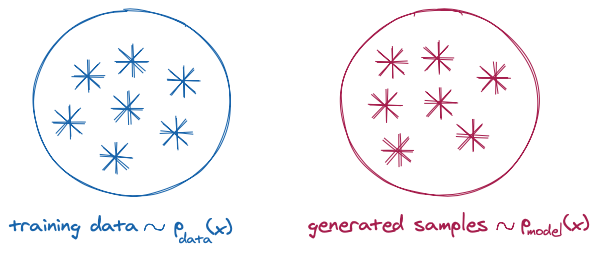
\includegraphics[scale=0.3]{../fig/density_estimation.png}
\end{figure}

\begin{center}
	\begin{minipage}{5cm}
		\begin{varblock}[5cm]{}
			\centering
			learn $p_{\text{model}}(x)$ close to $p_{\text{data}}(x)$
		\end{varblock}
	\end{minipage}
\end{center}

\end{frame}

\begin{frame}
	\frametitle{Density estimation}
	
\bit
\item core problem in the \textbf{unsupervised} learning setting
\item explicit: explicitly define and solve $p_{\text{model}}(x)$ 
\item implicit: learn a model that can sample from $p_{\text{model}}(x)$ without explicitly defining it
\eit

%goal: learn some underlying hidden \textbf{structure} of the data \\
%$\rightarrow$ \textit{clustering, dimensionality reduction, density estimation}

\end{frame}

\section{Variational Auto Encoders}

\begin{frame}
\frametitle{Auto encoders}

unsupervised approach for learning a lower dimensional feature representation \textbf{z} from unlabeled training data $x$

\begin{figure}
	\centering
	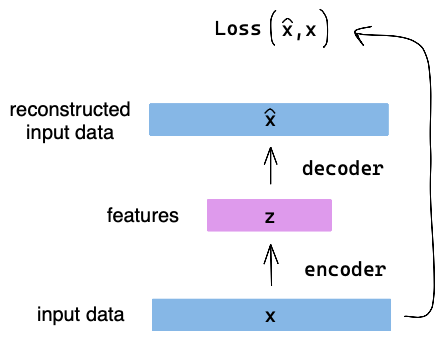
\includegraphics[scale=0.3]{../fig/ae.png}
\end{figure}

\textbf{z} captures meaningful factors of variation in the data\\

\vspace{3mm}
\centering
\textbf{Question: can we generate new images from an auto encoder?}

\end{frame}

\begin{frame}{Variational auto encoders}

VAEs are a probabilistic spin on auto encoders that will let us sample from the model to generate data\\

\vspace{2mm}

Assumption: training data $\{ x_i \}_{i \in [1,N]}$ is generated from underlying (latent) \textbf{unobserved} representation \textbf{z}\\

\vspace{5mm}

\begin{columns}
	\column{0.4\linewidth}
	\centering
	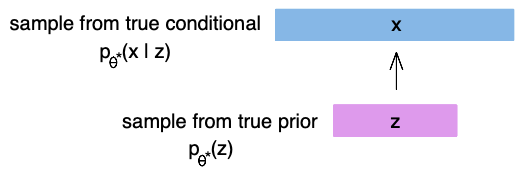
\includegraphics[width=5cm]{../fig/x_from_z.png}
	\column{0.4\linewidth}
	\textbf{Goal:} estimate the true parameters $\theta^*$ of this generative model
\end{columns} 

\vspace{5mm}

Choose simple prior $p(z)$ (e.g. Gaussian)\\
Conditional $p(x \vert z)$ is \textbf{complex}: represent it with a neural network\\

\vspace{3mm}
\centering
\textbf{Question: how do we train the model?}

\end{frame}

\begin{frame}{Intractability}

Natural strategy: learn model parameters to maximize the likelihood of the training data

\begin{align*}
	p_{\theta}(x) = \int p_{\theta}(x \vert \textbf{z}) p_{\theta}(\textbf{z}) d\textbf{z}
\end{align*}

Though we know $p_{\theta}(x \vert \textbf{z})$ and $p_{\theta}(\textbf{z})$, it is \textbf{intractable} to compute $p_{\theta}(x \vert \textbf{z})$ for every $z$!\\

\vspace{3mm}

Posterior density is also \textbf{intractable}: 

\begin{align*}
	p_{\theta}(\textbf{z} \vert x) = \dfrac{p_{\theta}(x \vert \textbf{z}) p_{\theta}(\textbf{z})}{p_{\theta}(x)} 
\end{align*}

\end{frame}

\begin{frame}
\frametitle{Solution}

In addition to the \textbf{decoder} network modeling $p_{\theta}(x \vert z)$, define an additional \textbf{encoder} network $q_{\delta}(z \vert x)$ that approximates  $p_{\theta}(z \vert x)$.\\

\begin{figure}
	\centering
	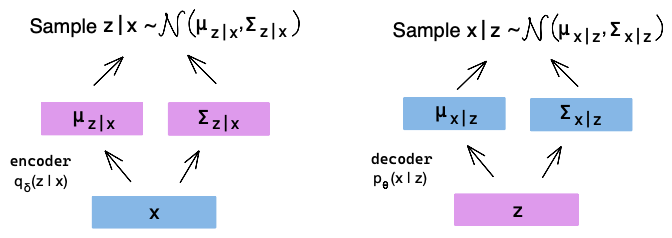
\includegraphics[scale=0.4]{../fig/p_and_q.png}
\end{figure}


This allows us to derive a \textbf{tractable} lower bound on the data likelihood

\end{frame}


\begin{frame} 
\frametitle{Tractable lower bound}

\begin{align*}
	\log p_{\theta}(x) & = \mathbb{E}_{z \sim q_\delta(z \vert x)} \big[ \log p_{\theta}(x) \big]\\
	& = \mathbb{E}_{z} \left[ \log \dfrac{p_{\theta}(x \vert z)p_{\theta}(z)}{p_{\theta}(z \vert x)} \right]\\
	& = \mathbb{E}_{z} \left[ \log \dfrac{p_{\theta}(x \vert z)p_{\theta}(z)}{p_{\theta}(z \vert x)} \dfrac{q_\delta(z \vert x)}{q_\delta(z \vert x)} \right]\\
	& = \mathbb{E}_{z} \left[ \log p_{\theta}(x \vert z) \right] - \mathbb{E}_{z} \left[ \log \dfrac{q_\delta(z \vert x)}{p_{\theta}(z)} \right] + \mathbb{E}_{z} \left[ \log \dfrac{q_\delta(z \vert x)}{p_{\theta}(z \vert x)} \right] \\
	& = \textcolor{Framavert}{ \mathbb{E}_{z} \left[ \log p_{\theta}(x \vert z) \right]} - \textcolor{Framableu}{d_{\text{KL}} \left( q_\delta(z \vert x) \vert \vert p_{\theta}(z) \right)} + \textcolor{Framaorange}{ d_{\text{KL}} \left( q_\delta(z \vert x) \vert \vert p_{\theta}(z \vert x) \right)} \\
\end{align*}

\end{frame}

\begin{frame}
\frametitle{Tractable lower bound}

- decoder network gives $p_\theta(x \vert z)$: we can estimate $\textcolor{Framavert}{ \mathbb{E}_{z} \left[ \log p_{\theta}(x \vert z) \right]}$ through sampling\\
- $\textcolor{Framableu}{d_{\text{KL}} \left( q_\delta(z \vert x) \vert \vert p_{\theta}(z) \right)}$ is the KL-div of two Gaussian distributions: it has a nice closed from solution\\
- though $p_\theta(z \vert x)$ is intractable, we know KL-div is always positive: $\textcolor{Framaorange}{ d_{\text{KL}} \left( q_\delta(z \vert x) \vert \vert p_{\theta}(z \vert x) \right)} \geq 0$\\

\vspace{5mm}

Hence,

\begin{align*}
	\log p_{\theta}(x) & \geq \textcolor{magenta}{ \mathbb{E}_{z} \left[ \log p_{\theta}(x \vert z) \right] - d_{\text{KL}} \left( q_\delta(z \vert x) \vert \vert p_{\theta}(z) \right) }\\
	& \geq \textcolor{magenta}{\mathcal{L} (x, \theta, \delta)}
\end{align*}

We've identified a \textbf{tractable} + \textbf{differentiable} lower bound which we can take gradient of and optimize (ELBO, evidence lower bound)

\end{frame}

\begin{frame}
\frametitle{Training}

Optimal parameters will be the ones that maximizes this lower bound: 

\begin{align*}
 \theta^*, \delta^* = \arg \max_{\theta, \delta} \sum_{i=1}^{N} \mathcal{L} (x_i, \theta, \delta)
\end{align*} 

\end{frame}

\begin{frame}
\frametitle{Training}

\begin{figure}
	\centering
	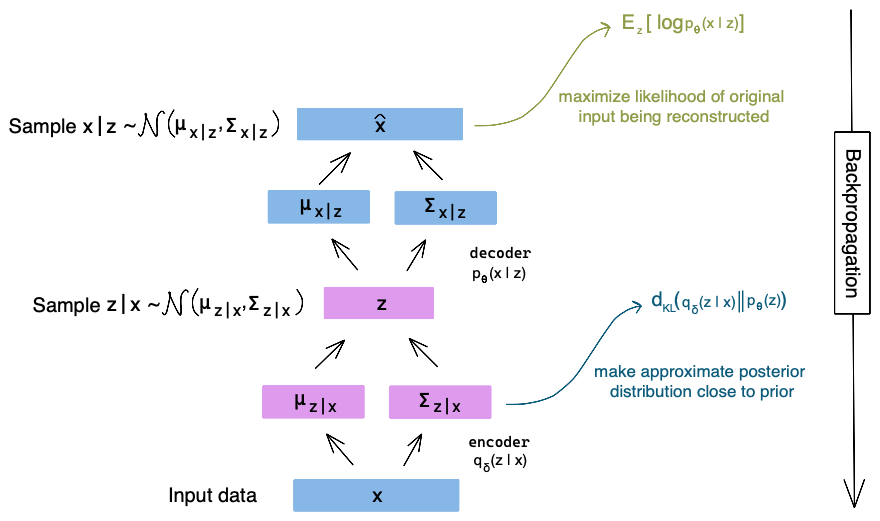
\includegraphics[scale=0.33]{../fig/vae.png}
\end{figure}

\end{frame}

\begin{frame}
\frametitle{Data generation}

Once trained, we can sample \textbf{z} from prior and use the decoder network to generate new data:

\begin{figure}
	\centering
	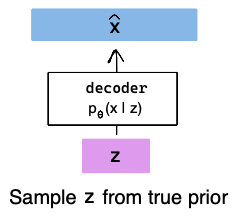
\includegraphics[scale=0.4]{../fig/generate_data.png}
\end{figure}

\end{frame}

\begin{frame}
Bibliography :

\vspace{2mm}

\nocite{*}
\small{\bibliographystyle{unsrt}
\bibliography{biblio}\vspace{0.75in}}

\end{frame}

\end{document}